%
% Complete documentation on the extended LaTeX markup used for Insight
% documentation is available in ``Documenting Insight'', which is part
% of the standard documentation for Insight.  It may be found online
% at:
%
%     http://www.itk.org/

\documentclass{InsightArticle}
\usepackage[american]{babel}
\usepackage[utf8]{inputenc}

\usepackage[super,sort&compress,comma]{natbib}

\usepackage[dvips]{graphicx}
%\usepackage[hyphens]{url}%does not work with hyperref


\usepackage{listings}% https://en.wikibooks.org/wiki/LaTeX/Source_Code_Listings
\lstset{basicstyle=\footnotesize\ttfamily,breaklines=true}% http://tex.stackexchange.com/questions/33685/set-the-font-family-for-lstlisting
\lstdefinelanguage{diff}{% http://tex.stackexchange.com/questions/50176/highlighting-a-diff-file#50263
  morecomment=[f][\color{blue}]{@@},     % group identifier
  morecomment=[f][\color{red}]-,         % deleted lines 
  morecomment=[f][\color{green}]+,       % added lines
  morecomment=[f][\color{magenta}]{---}, % Diff header lines (must appear after +,-)
  morecomment=[f][\color{magenta}]{+++},
}


%%%%%%%%%%%%%%%%%%%%%%%%%%%%%%%%%%%%%%%%%%%%%%%%%%%%%%%%%%%%%%%%%%
%
%  hyperref should be the last package to be loaded.
%
%%%%%%%%%%%%%%%%%%%%%%%%%%%%%%%%%%%%%%%%%%%%%%%%%%%%%%%%%%%%%%%%%%
%\PassOptionsToPackage{hyphens}{url}\%does not make a difference
\usepackage[%dvips,%prevents internal pdf-links -> use pdflatex!
bookmarks,
bookmarksopen,
backref,
colorlinks,linkcolor={blue},citecolor={blue},urlcolor={blue},
]{hyperref}


\hyphenation{pre-ser-ving di-gi-tal}


%  This is a template for Papers to the Insight Journal.
%  It is comparable to a technical report format.

% The title should be descriptive enough for people to be able to find
% the relevant document.
\title{Providing neighbouring voxel values by vtkDiscreteMarchingCubes}

%
% NOTE: This is the last number of the "handle" URL that
% The Insight Journal assigns to your paper as part of the
% submission process. Please replace the number "1338" with
% the actual handle number that you get assigned.
%
\newcommand{\IJhandlerIDnumber}{xxxx}

% Increment the release number whenever significant changes are made.
% The author and/or editor can define 'significant' however they like.
\release{1.00}

% At minimum, give your name and an email address.  You can include a
% snail-mail address if you like.
\author{Roman Grothausmann$^{1}$}
\authoraddress{$^{1}$grothausmann.roman@mh-hannover.de,\\ 
                     Institute of Functional and Applied Anatomy,
                     Hannover Medical School and\\%, Hannover, Germany\\ 
                     REBIRTH Cluster of Excellence, Hannover, Germany
}

\sloppy


\begin{document}

%
% Add hyperlink to the web location and license of the paper.
% The argument of this command is the handler identifier given
% by the Insight Journal to this paper.
%
\IJhandlefooter{\IJhandlerIDnumber}


\ifpdf
\else
   %
   % Commands for including Graphics when using latex
   %
   \DeclareGraphicsExtensions{.eps,.jpg,.gif,.tiff,.bmp,.png}
   \DeclareGraphicsRule{.jpg}{eps}{.jpg.bb}{`convert #1 eps:-}
   \DeclareGraphicsRule{.gif}{eps}{.gif.bb}{`convert #1 eps:-}
   \DeclareGraphicsRule{.tiff}{eps}{.tiff.bb}{`convert #1 eps:-}
   \DeclareGraphicsRule{.bmp}{eps}{.bmp.bb}{`convert #1 eps:-}
   \DeclareGraphicsRule{.png}{eps}{.png.bb}{`convert #1 eps:-}
\fi


\maketitle


\ifhtml
\chapter*{Front Matter\label{front}}
\fi


% The abstract should be a paragraph or two long, and describe the
% scope of the document.
\begin{abstract}
\noindent
The contribution to VTK presented in this article is an extension to \code{vtkDiscreteMarchingCubes} to also create \code{vtkPointData} scalars containing the value of the neighbouring voxel. These can be used to remove regions of the maching-cubes\citep{Lorensen1987} mesh depending on the local neighbourhood.
The extension is based on the code of \code{vtkDiscreteMarchingCubes} of VTK-6.3.0 and is available on GitLab \url{https://gitlab.kitware.com/vtk/vtk/merge_requests/889} (and GitHub \url{https://github.com/Kitware/VTK/pull/18}).
\end{abstract}

\IJhandlenote{\IJhandlerIDnumber}

\tableofcontents

\pagebreak

\section{Introduction}


\begin{figure}[!b]
\center
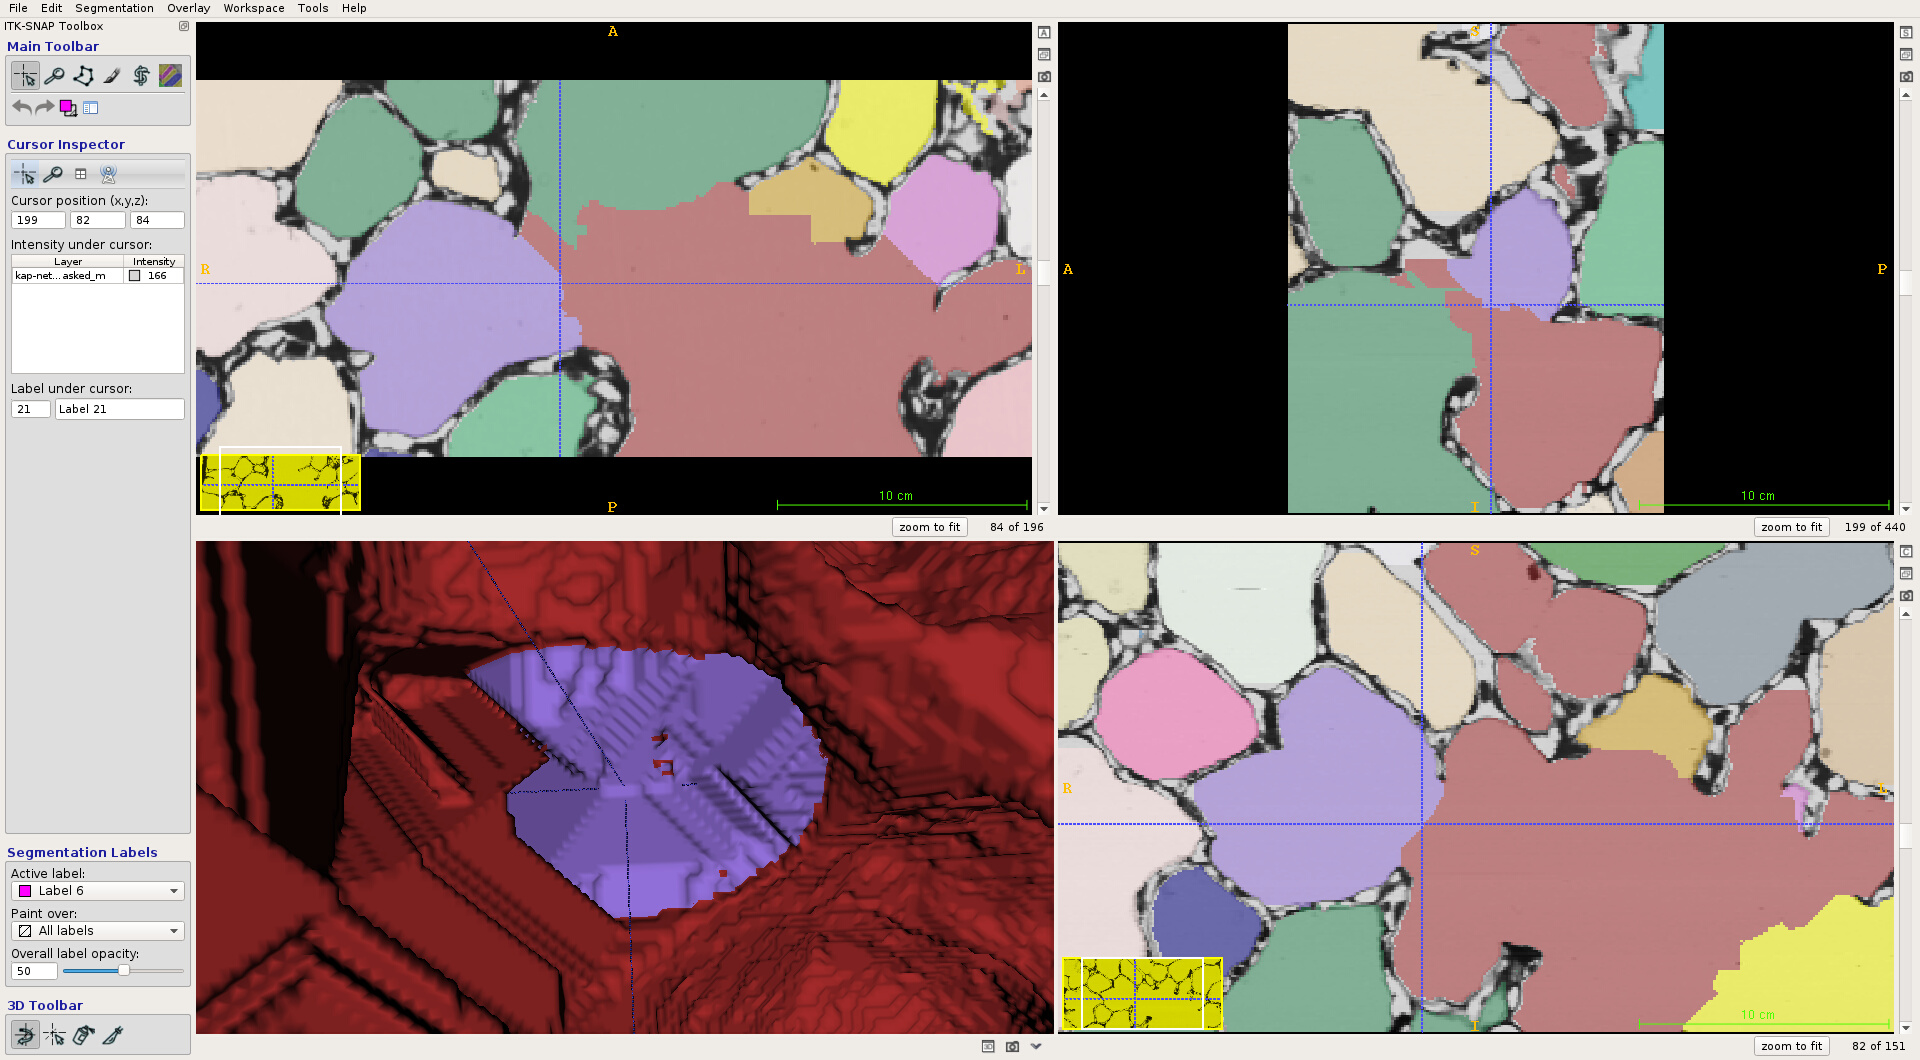
\includegraphics[width=\textwidth]{images/vtkDiscreteMarchingCubes_extension_07}
\itkcaption[]{
Segmentation with touching labels\\
\footnotesize
Slices of a label image that separates a segmentation at constrictions and also contains a background label (0, rendered fully transparent). The cursor is on label 21 (light purple) which is adjacent to label 19 (dark pink). This is a screenshot of ITKSnap\citep{itksnap,Yushkevich2006}.
}
\label{fig:labelimage}
\end{figure}


This extension to \code{vtkDiscreteMarchingCubes} makes it possible to let \code{vtkDiscreteMarchingCubes} also create \code{vtkPointData} scalars containing the label value of the neighbouring voxel in a label image. This then allows to remove regions of the resulting mesh that are adjacent to specific labels. For example a label image as in Fig.~\ref{fig:labelimage} that was created by running a watershed on a distance map followed by masking with the original binary segmentation, a common procedure to separate regions in a binary image at constrictions (see e.g. \citet{Beare2006b}). Such a label image is shown in Fig.~\ref{fig:labelimage}.

When creating meshes for each foreground label from such a label image the meshes are closed at the constrictions where the separation was introduced, see 3D view in Fig.~\ref{fig:labelimage} and Fig.~\ref{fig:dmcCO}.

With the contributed extension to \code{vtkDiscreteMarchingCubes} the resulting mesh contains additional scalar data for the points that holds the label value of the adjacent label. A simple threshold that extracts the regions of the meshes that are adjacent to the background label (0) then makes it possible to remove the capping at constrictions, see Fig.~\ref{fig:dmcCO}.

For example looking at label 19 and 21 (extracted by a simple threshold on the cell scalars generated by \code{vtkDiscreteMarchingCubes}) which are adjacent to each other but mostly separated by the background label, see Fig.~\ref{fig:dmcCOt21t19}.

An additional threshold on the point scalars then removes the capping at the separation, see Fig.~\ref{fig:dmcCOt21t19}.

\begin{figure}[p]
\center
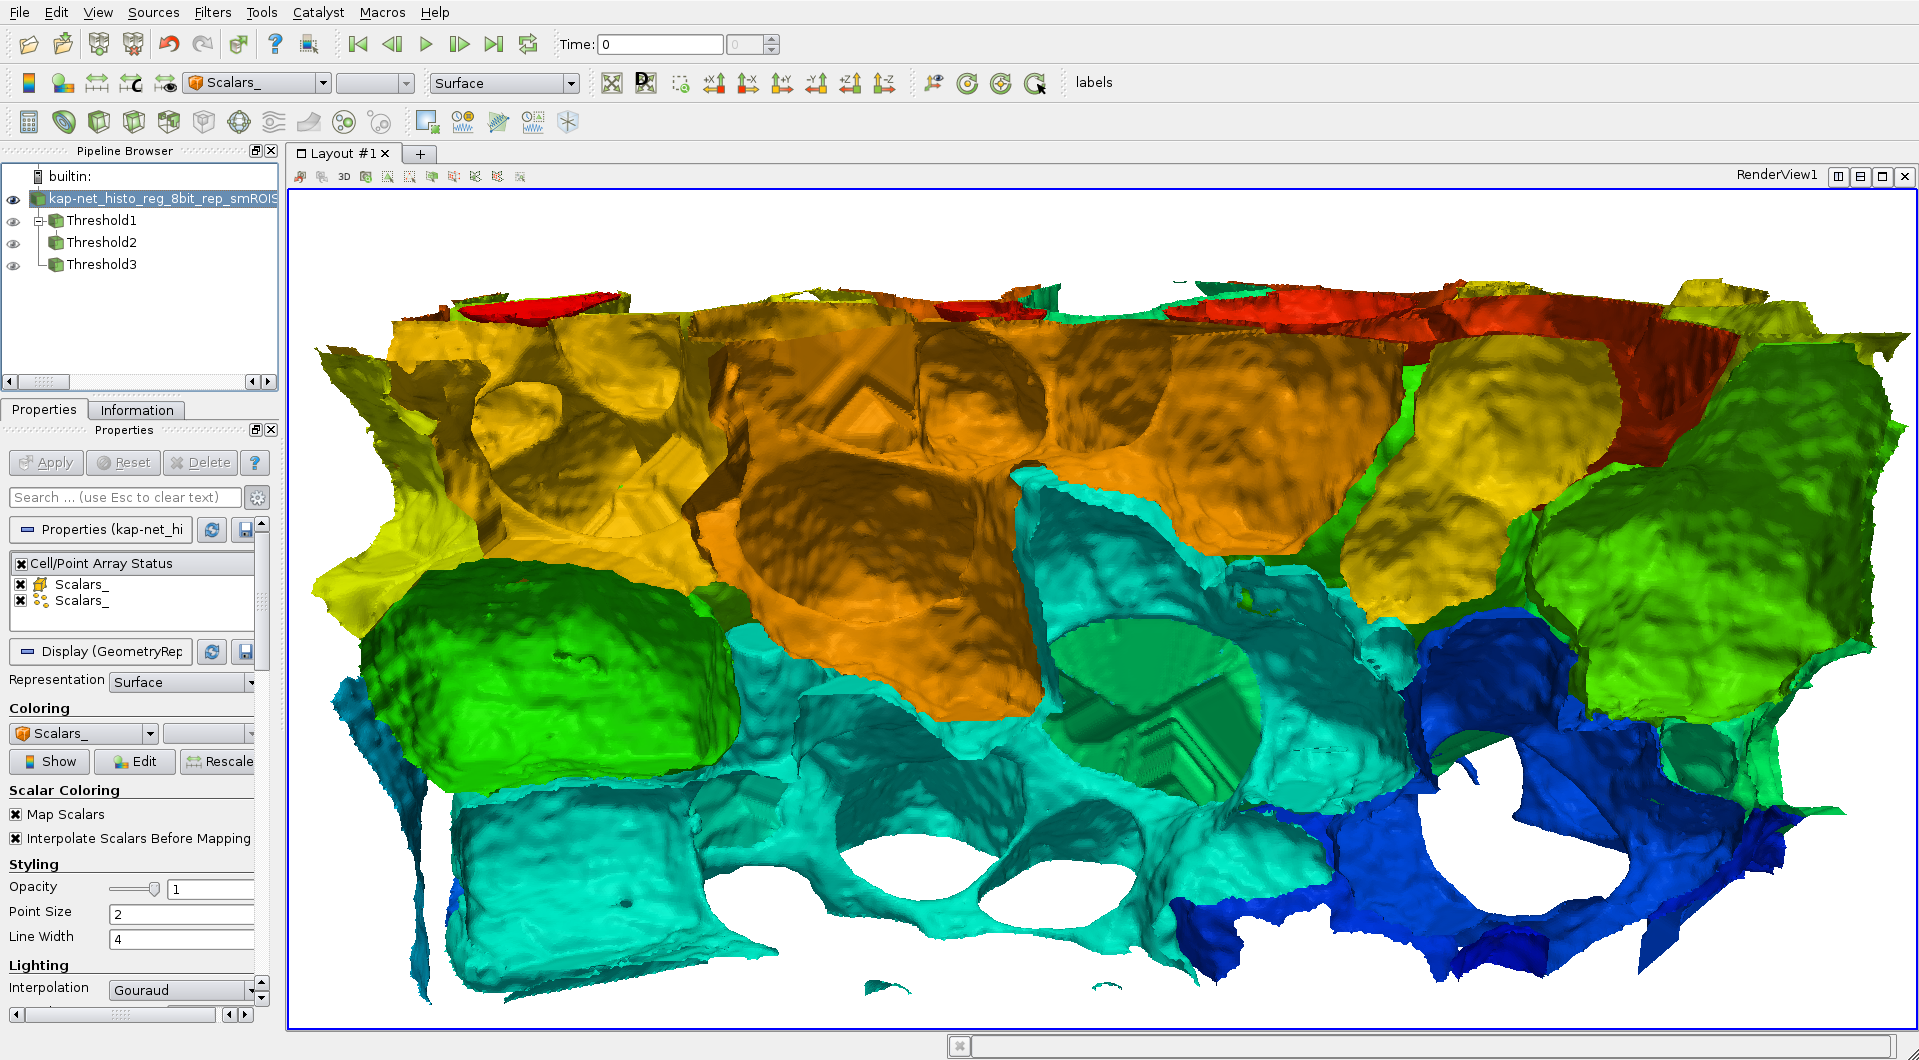
\includegraphics[width=.48\textwidth]{images/vtkDiscreteMarchingCubes_extension_01}
\hfill
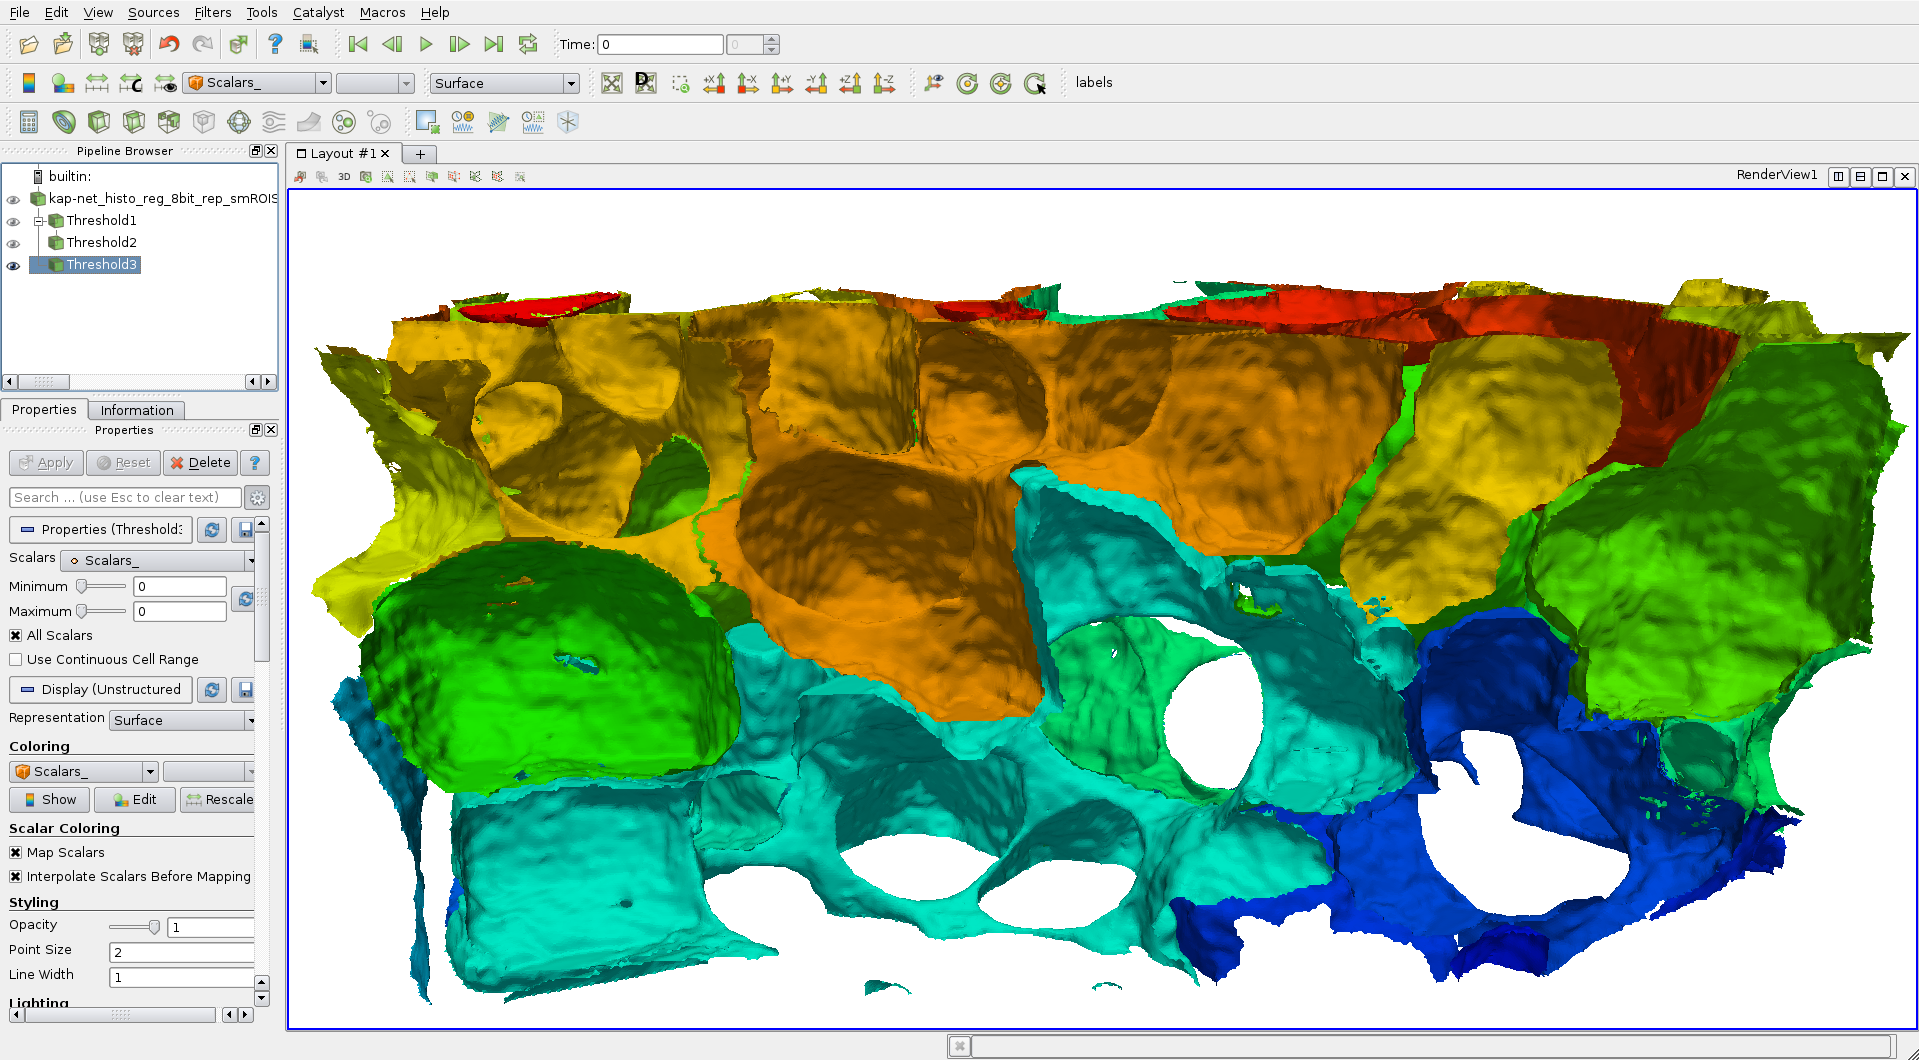
\includegraphics[width=.48\textwidth]{images/vtkDiscreteMarchingCubes_extension_02}
\itkcaption[]{
\\
\footnotesize
left: Meshes generated by \code{vtkDiscreteMarchingCubes} for the label image shown above, coloured differently and smoothed with \code{vtkWindowedSincPolyDataFilter}. Note the capping at constrictions.\\
right: Result only displaying those regions of the meshes that were adjacent to the background label. Note that the capping is removed.
}
\label{fig:dmcCO}
\end{figure}

\begin{figure}[p]
\center
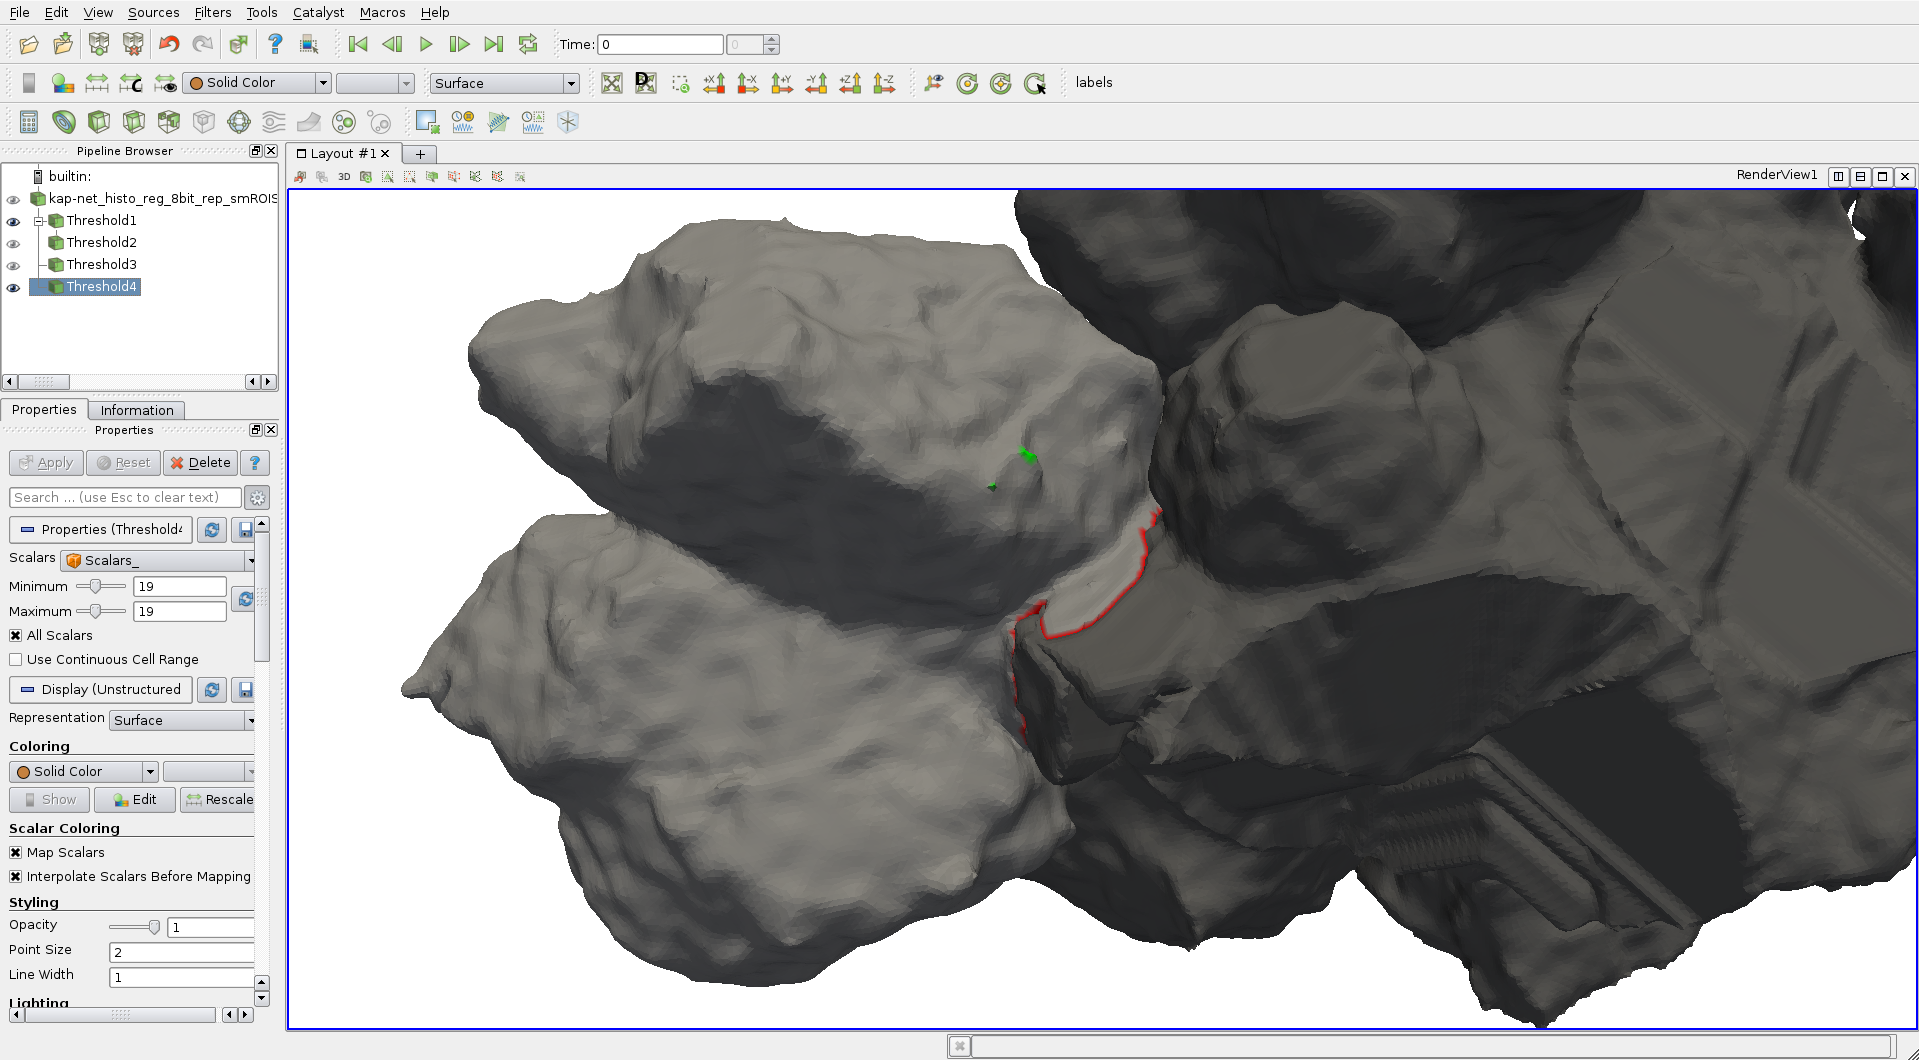
\includegraphics[width=.48\textwidth]{images/vtkDiscreteMarchingCubes_extension_03}
\hfill
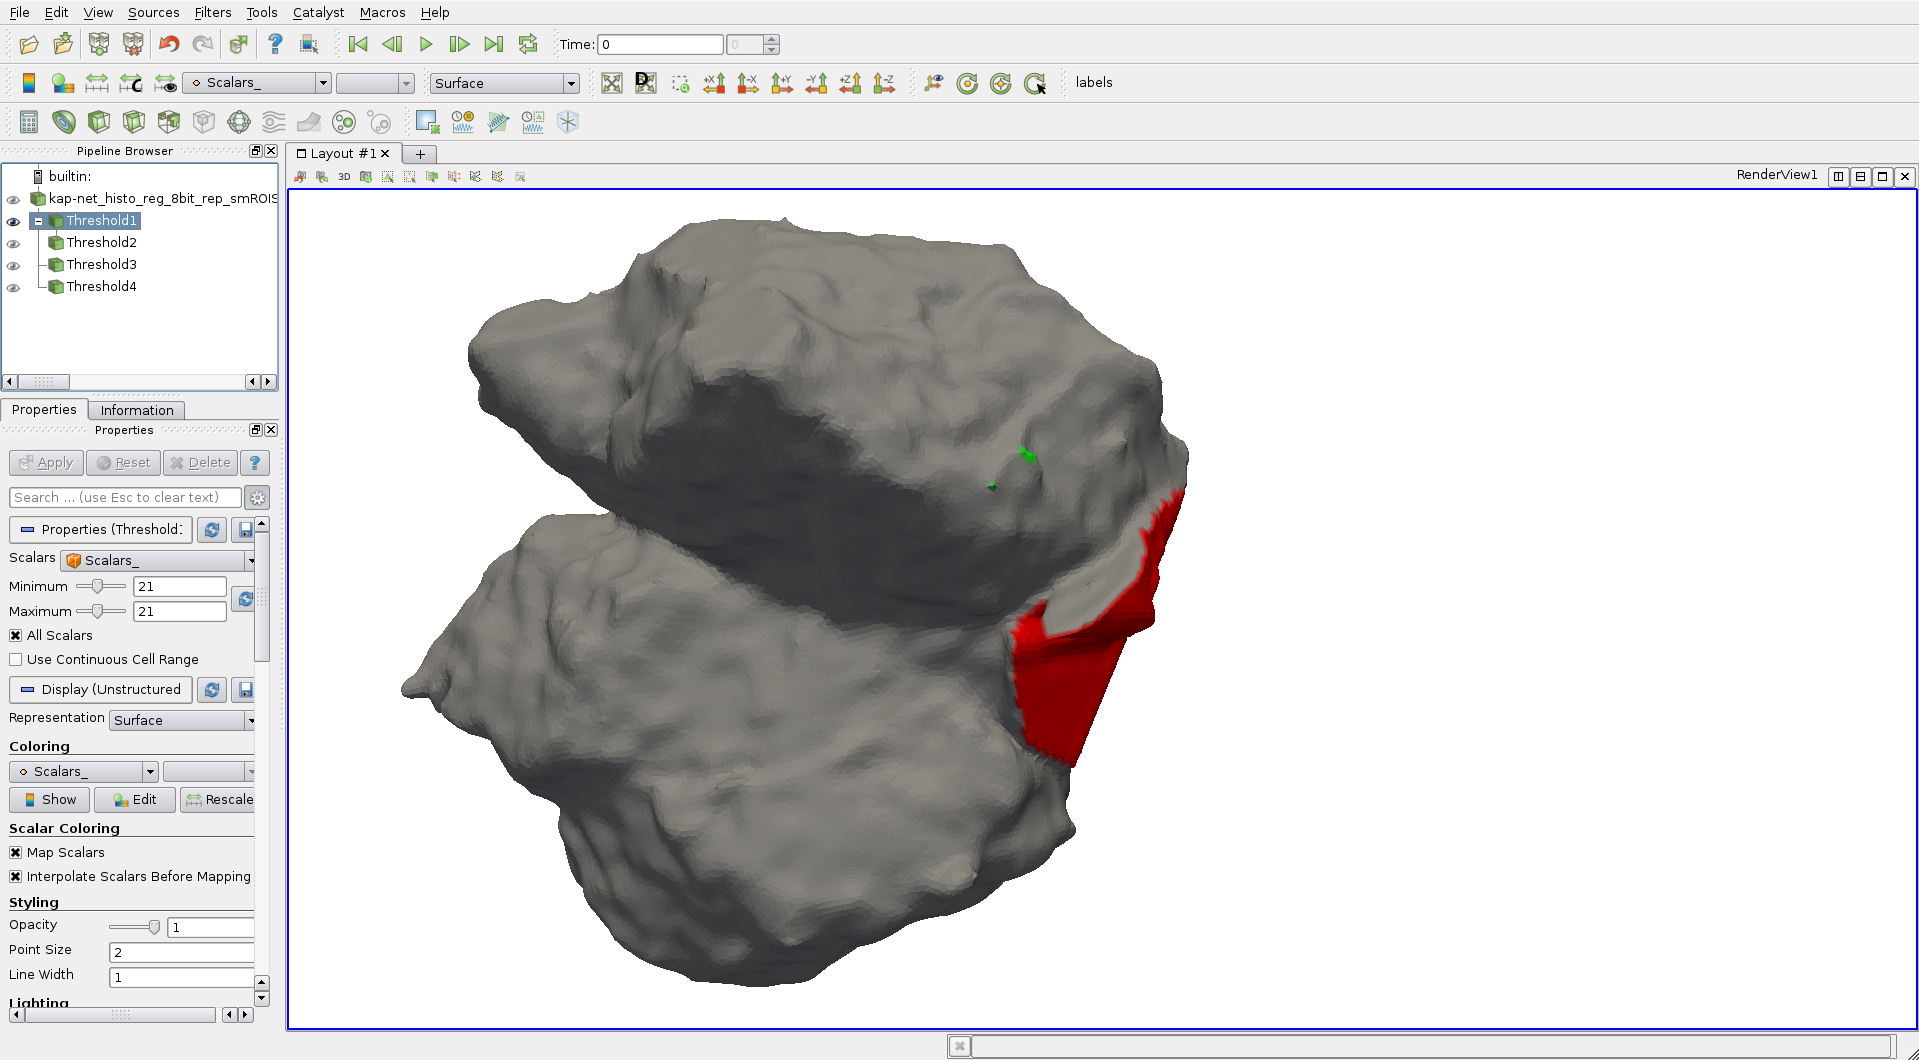
\includegraphics[width=.48\textwidth]{images/vtkDiscreteMarchingCubes_extension_04}
\\[5mm]
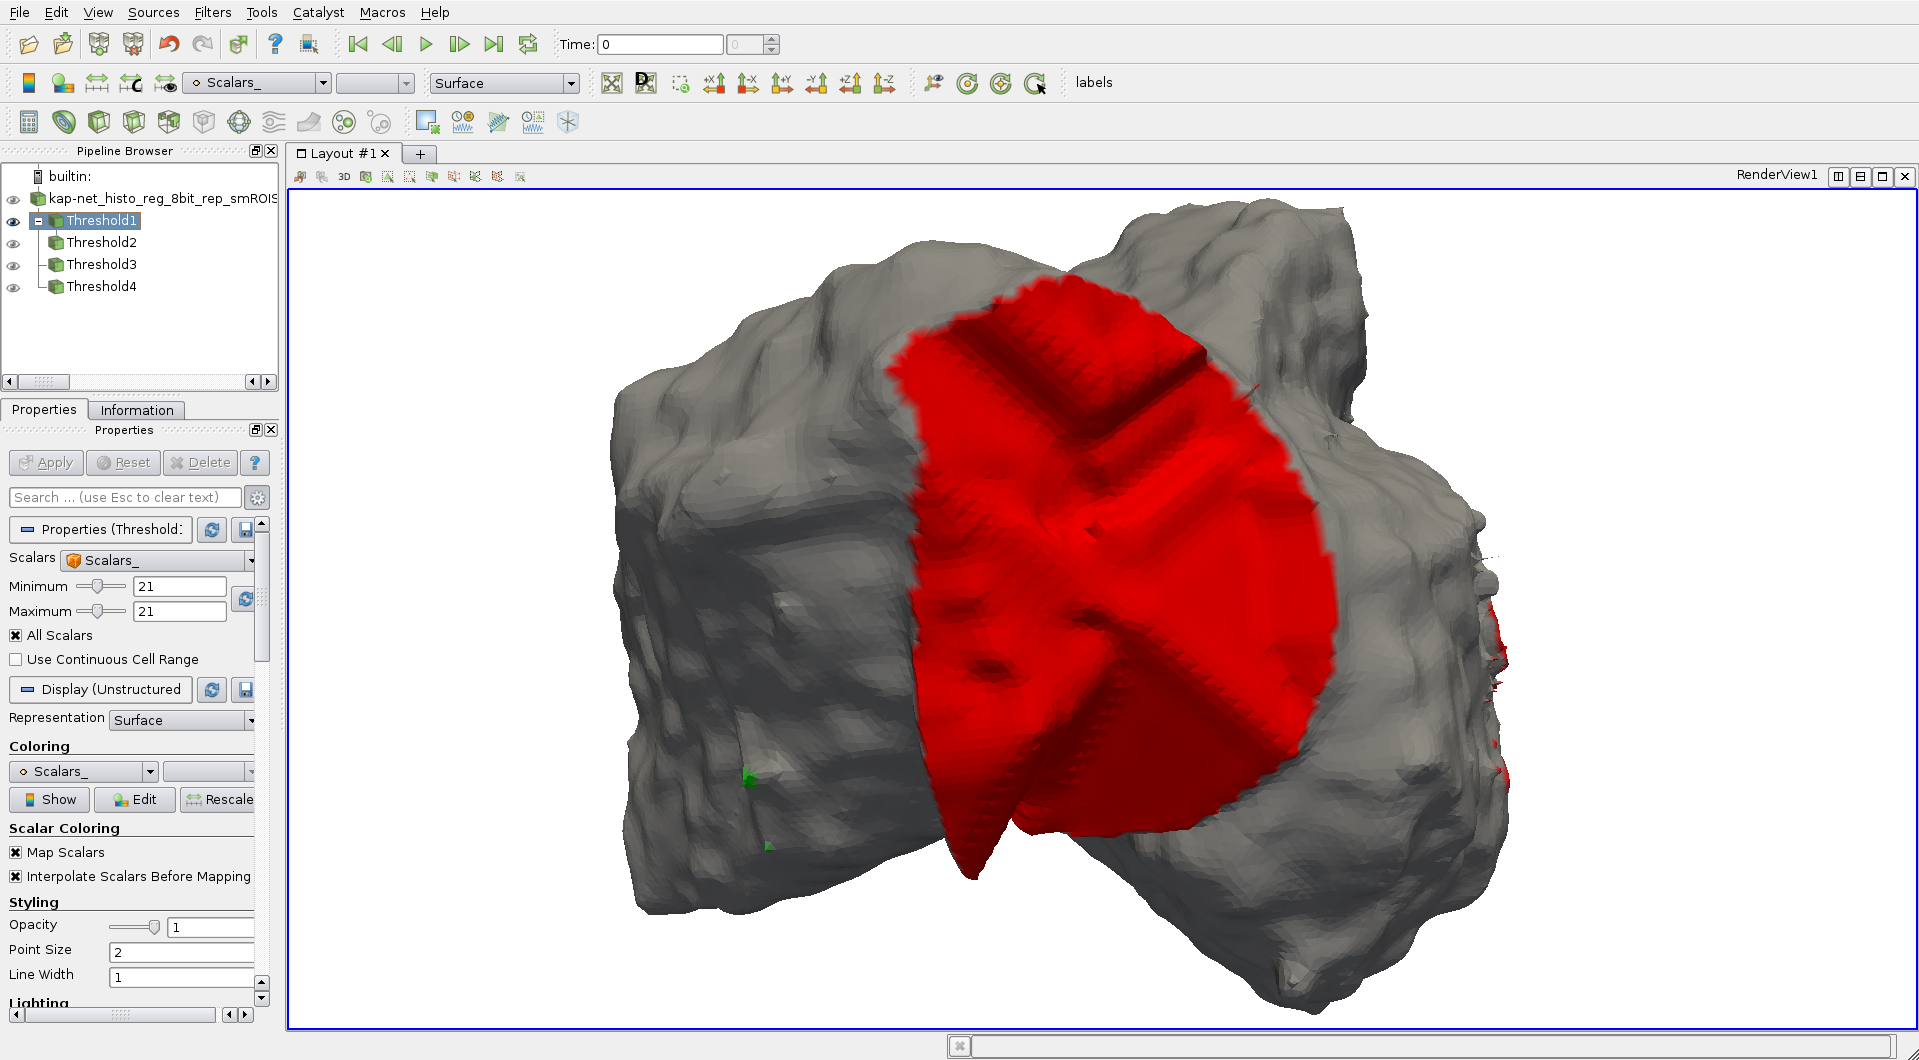
\includegraphics[width=.48\textwidth]{images/vtkDiscreteMarchingCubes_extension_05}
\hfill
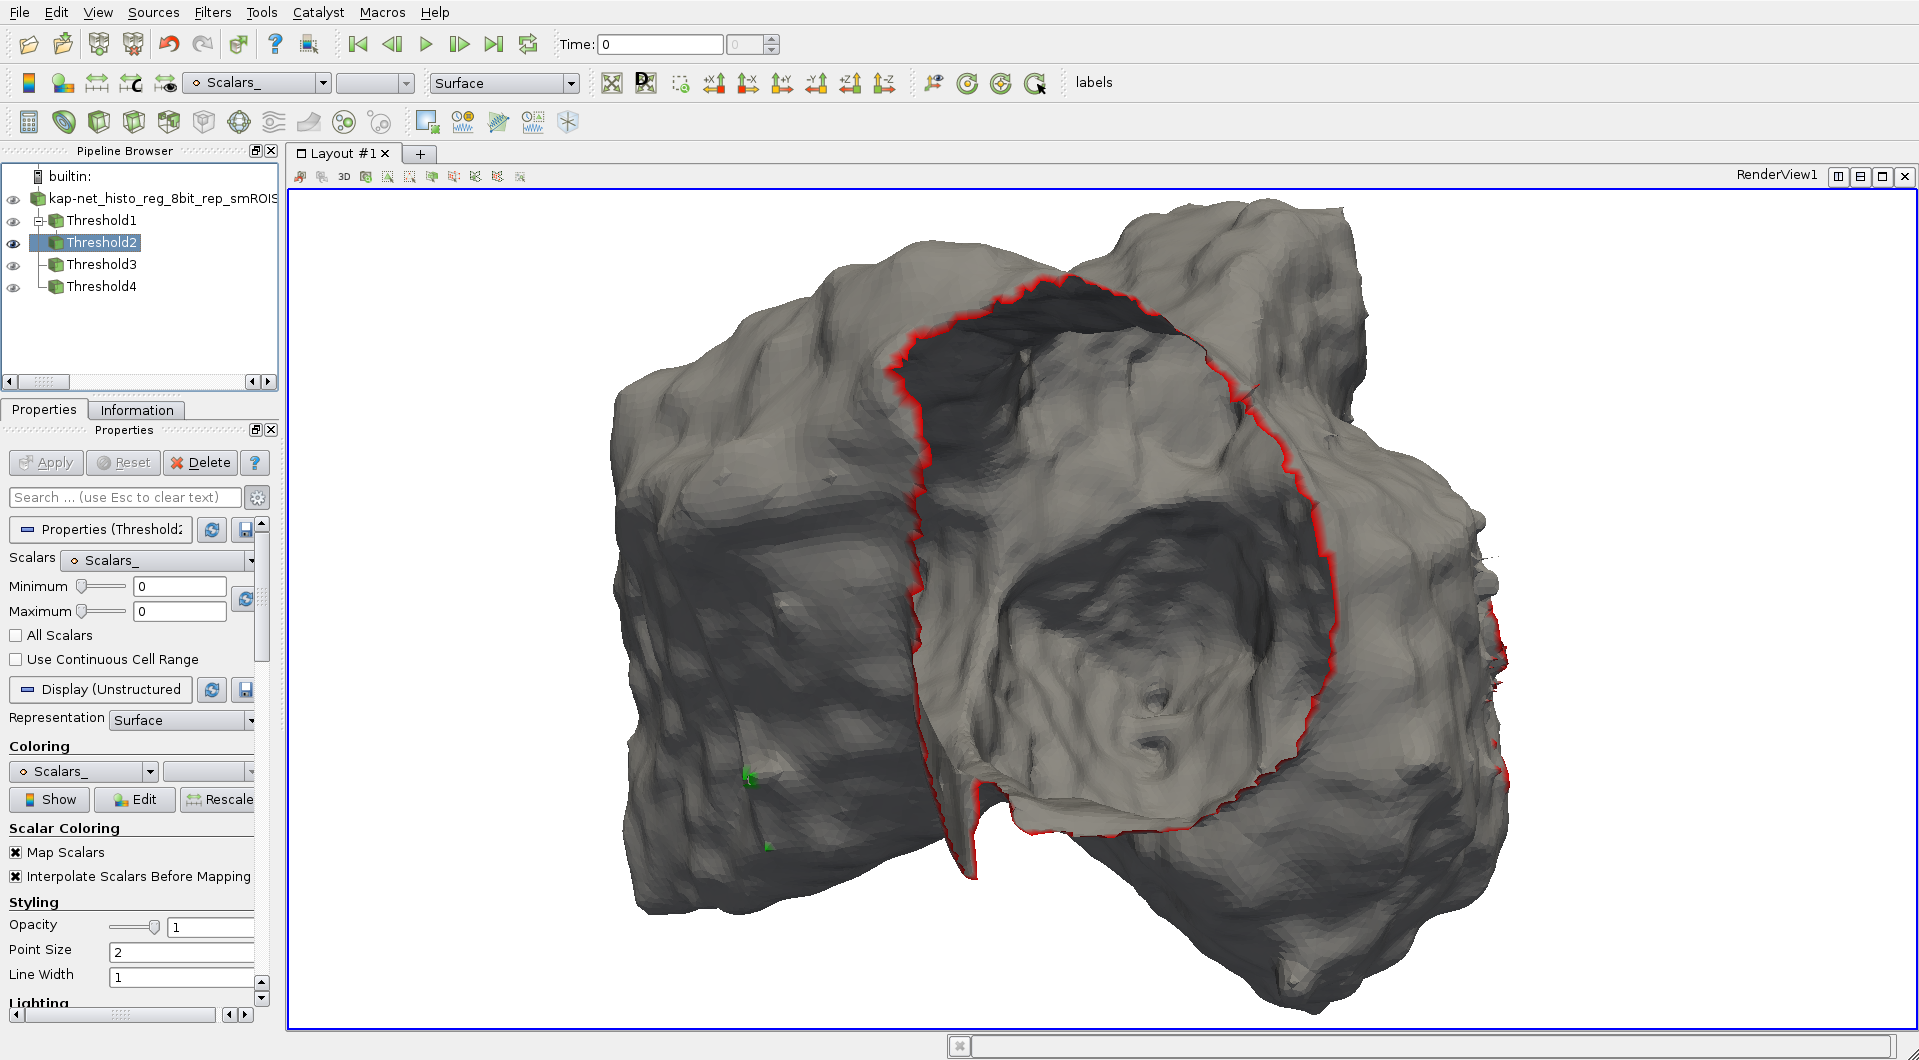
\includegraphics[width=.48\textwidth]{images/vtkDiscreteMarchingCubes_extension_06}
\itkcaption[]{
\\
\footnotesize
Showing only the meshes of label 21 (light grey) and 19 (dark grey) (top left). Regions of the mesh of label 21 are coloured if adjacent to other labels, e.g. red where 19 and 21 touch, i.e. where the separation took place.
Other images show views of label 21 only,
in the bottom left the capping is removed.
}
\label{fig:dmcCOt21t19}
\end{figure}


An advantage of this kind of capping removal is that it is even possible after the mesh was modified by other filters, e.g. smoothed by \code{vtkWindowedSincPolyDataFilter}. However, in most cases the resulting meshes are not connected on the open border edges any more, i.e. there will be gaps between them. The \code{vtkCoplanarSurfaceExtractor}\citep{Grothausmann2014_r} can be used to avoid such gaps.



\section{Implementation}
\label{sec:impl}


Below the partial listing of the patch that contains the essential changes to \code{vtkDiscreteMarchingCubes.cxx}:

\lstinputlisting[language=diff,
  linerange={% http://tex.stackexchange.com/questions/34323/using-lstinputlisting-to-include-a-file-but-only-certain-lines-or-line-ranges#34325
    1-4
    ,36-58
    %% ,67-83
    %% ,100-112
  }
]{diffs/vtkDiscreteMarchingCubes.cxx_b02cbff0f1..bb8e3caf71.gitdiff}% VTK$ git diff b02cbff0f1 bb8e3caf71  Filters/General/vtkDiscreteMarchingCubes.cxx > $@



\section{Testing (usage example)}
\label{sec:test}


A test based on \code{TestDiscreteMarchingCube.py} was created to monitor the newly added functionality:

\lstinputlisting[language=diff,
]{diffs/TestDiscreteMarchingCubesAdjacentScalars.py_f4c02685b4..5b5e5add65.gitdiff}% VTK$ git diff f4c02685b4 5b5e5add65  Filters/General/Testing/Python/TestDiscreteMarchingCubesAdjacentScalars.py > $@



%\pagebreak

%%%%%%%%%%%%%%%%%%%%%%%%%%%%%%%%%%%%%%%%%
%
%  Insert the bibliography using BibTeX
%
%%%%%%%%%%%%%%%%%%%%%%%%%%%%%%%%%%%%%%%%%

%\sloppy%does not cause URL to break
%\renewcommand{\UrlBreaks}{\do\/\do\a\do\b\do\c\do\d\do\e\do\f\do\g\do\h\do\i\do\j\do\k\do\l\do\m\do\n\do\o\do\p\do\q\do\r\do\s\do\t\do\u\do\v\do\w\do\x\do\y\do\z\do\A\do\B\do\C\do\D\do\E\do\F\do\G\do\H\do\I\do\J\do\K\do\L\do\M\do\N\do\O\do\P\do\Q\do\R\do\S\do\T\do\U\do\V\do\W\do\X\do\Y\do\Z}%breaks long URLs
\renewcommand{\UrlBreaks}{\do\-\do\_}%breaks long URLs also at hyphens
%\bibliographystyle{plainnat}
\bibliographystyle{unsrtnat}%to check the order of the citations
\bibliography{vtkDiscreteMarchingCubes_extension}


\end{document}

